%%
%% sample.tex
%%   example of use of the ACESJournal LaTex template for ACES journals (http://www.aces-society.org/)
%%
%% Copyright (c) 2016 by Luca De Camillis
%%
%% Authors:
%%   Luca De Camillis <lucadecamillis@gmail.com>
%%
%% License:
%%   This Source Code Form is subject to the terms of the Mozilla Public
%%   License, v. 2.0. If a copy of the MPL was not distributed with this
%%   file, You can obtain one at http://mozilla.org/MPL/2.0/.
%%
%%   This Source Code Form is 'Incompatible With Secondary Licenses',
%%   as defined by the Mozilla Public License, v. 2.0.
%%



\documentclass[letterpaper,twocolumn]{ACESJournal}
\usepackage[utf8]{inputenc}
\usepackage[T1]{fontenc}
\usepackage{microtype}
\usepackage{times}

%
\usepackage{color}
\usepackage{graphicx}
\usepackage{tabularx}
%
\newcommand{\red}[1]{{\color{red}#1}}
%
\title{Author Guidelines for ACES Journal Papers \red{(14 pt bold)}}
%
\author{Author O. Lastname, Author T. Lastname, and Author T. Lastname\\%
\red{(12 pt bold; author's names should be listed by the full first name, middle initial, and last name)}}
%
\affiliation{Department of Electrical Engineering (\red{10 pt plain text})\\%
University of Electromagnetics, City, State Code Zip Code, Country\\%
first author email, third author email (\red{No underlines below email addresses})}
%
\affiliation{Department of Electrical and Computer Engineering\\%
Antenna Design University, City, State Code Zip Code, Country\\%
second author (\red{No underlines below email addresses})}
%
\begin{document}
%
\maketitle
%
\begin{abstract}
The abstract should convey the general ideas of the paper in a clear and concise form. It should be a \red{single short paragraph} that indicates to the reader the subject matter being presented. \red{All submitted papers should be formatted to $8.5 \times 11$ inch ($21.6 \times 27.9$ cm) paper size and complying with the specified font sizes listed here.} Use this document as a template if you are using Microsoft Word 6.0 or later. Otherwise, use this document as an instruction set. It is important to maintain the highest quality of figures and text throughout the paper. \red{A paper will be accepted for publication only when it contains material that is neat, legible, reproducible, and in accordance with the format detailed in this template.}
\end{abstract}
%
\begin{ACESkeywords}
List key words or phrases \red{in alphabetical order}, separated by commas and \red{ending with a period}.
\end{ACESkeywords}
%
\section{INTRODUCTION}
\label{sec:INTRODUCTION}
%
The paper title, author(s), abstract, and the beginning of the paper itself should all be on the first page. The \red{paper} title, author(s), and author affiliations should be centered \red{(center-justified)} on the first page. The title should be of font size 14 pt and bolded, the author names should be of font size 12 pt and bolded, and the author affiliation should be of font size 10 pt \red{(regular Times New Roman font, neither italic nor bolded in the affiliation). There should be two blank lines (10 pt) between title and author(s), one blank line (10 pt) between author(s) and affiliation, and one blank line (10 pt) between different affiliations. Two blank lines should be left between last affiliations and the abstract and general text (10 pt)}.

General text of the paper, \red{starting with the abstract}, should be of font size \red{10 pt}, Times New Roman font, single line spacing, and arranged in two columns. \red{Both columns should be fully justified, and the beginnings of the two columns in each page should be aligned vertically. All page margins should be 1 inch, except for the first page, where the TITLE should be 1.5 inches below the top of the page (use the paragraph settings to set the space before to 24 pt)}.

Unused space should be minimized. Proper formatting is essential to a speedy processing of technically accepted papers for final acceptance and printing.

An abstract is required, which should be a brief summary of the work described in the paper. It should state the computer codes, computational techniques, and applications discussed in the paper (as applicable) and should otherwise be usable by technical abstracting and indexing services. \red{References should not be included in the abstract section.} The word ``Abstract'' and ``Index Terms'' must be placed at the left margin of the paper, and should be \red{bolded} and \red{italic}. It also should be followed by a long hyphen or \textit{m}-dash (--) with the main text of the abstract and index terms starting on the same line. \red{Leave a space before and after the hyphen.} Either British English or American English spellings may be used, provided that each word is spelled consistently throughout the paper. The intent and meaning of all text must be clear. For authors who are not masters of the English language, the ACES Editorial Staff will provide assistance with grammar (subject to clarity of intent and meaning). However, this may delay the scheduled publication date.

It is the author(s) responsibility to provide acceptable files for printing. Incompatible or incomplete files will not be processed for publication, and authors will be requested to re-upload a revised acceptable version. If needed, ACES reserves the right to edit any submitted material.
%
\section{SECTION FORMATTING}
%
All section titles should be centered and all the title letters should be written in capital letters. \red{Section titles should be of size 11 pt, bolded and center-justified.} The section titles need to be numbered using Roman numerals (I. II. \ldots). Sections and subsections should not normally begin on a new page or a new column. All new paragraphs should be indented with a quarter inch (in the paragraph settings, set indentation of first line to 0.25). One line space should separate the end of a previous section, and the next section's title.
%
\subsection{Subsection title formatting}
%
Subsection titles should be numbered with Roman uppercase letters (A. B. \ldots). Only the first word of the subsection title should be capitalized.
%
\subsection{Subsection title formatting continued}
%
Subsection titles should be written in \red{bold 10 pt font and fully justified}. One line space should separate the end of a previous subsection with the next subsection or section’s title.
%
\section{FORMATTING OF EQUATIONS, FIGURES, AND REFERENCES}
%
\subsection{Equation formatting}
%
Internal consistency should be maintained regarding elements of style such as equation numbering. Equation numbers should be in sequential and placed in parentheses at the right margin of each column. \red{Each equation should end in a period or comma}. An example is shown below where the equation represents the end of a sentence.
%
\begin{equation}
\label{eq:diff}
x^{2} \, y^{''} + x \, y^{'} + \left( x^{2} - v^{2} \right) y = 0.
\end{equation}
%
\red{Another example is as follows:}
%
\begin{equation}
\label{eq:wavelength}
\lambda = c / f,
\end{equation}
%
where $\lambda$ is the wavelength, $c$ is the speed of light in free space, and $f$ is the frequency. Notice that equation (\ref{eq:diff}) ends with a ``.'', while equation (\ref{eq:wavelength}) ends with a ``,''.
%
\subsection{Figure and table formatting}
%
Figures and tables should be formatted appropriately (centered within the column, side-by-side, etc.) on the page such that the presented data appears close to and after it is first referenced in the text. When including figures and tables, care should be taken so that they will appear appropriately when printed in black and white. \red{For better visibility of plots on a computer screen, it is recommended to use different line styles for color figures with multiple curves such as in Fig. \ref{fig:power_reflection}}. Colors should also be tested to insure their ability to be distinguished after black and white printing. \red{Avoid the use of large symbols with curves in a figure}. Figures with multiple curves should use different line styles such as solid, dotted, dashed, etc.

\red{A figure caption should be located directly beneath the corresponding figure, and should be fully justified. Figure captions should be written in the following form ``Fig. \#. Description of the figure.'', as illustrated by Fig. \ref{fig:power_reflection} below. Each caption should end with a period.} All figures should have white background. Do not include a bounding box surrounding a figure.
%
\begin{figure}%[!htb]
  \begin{center}
  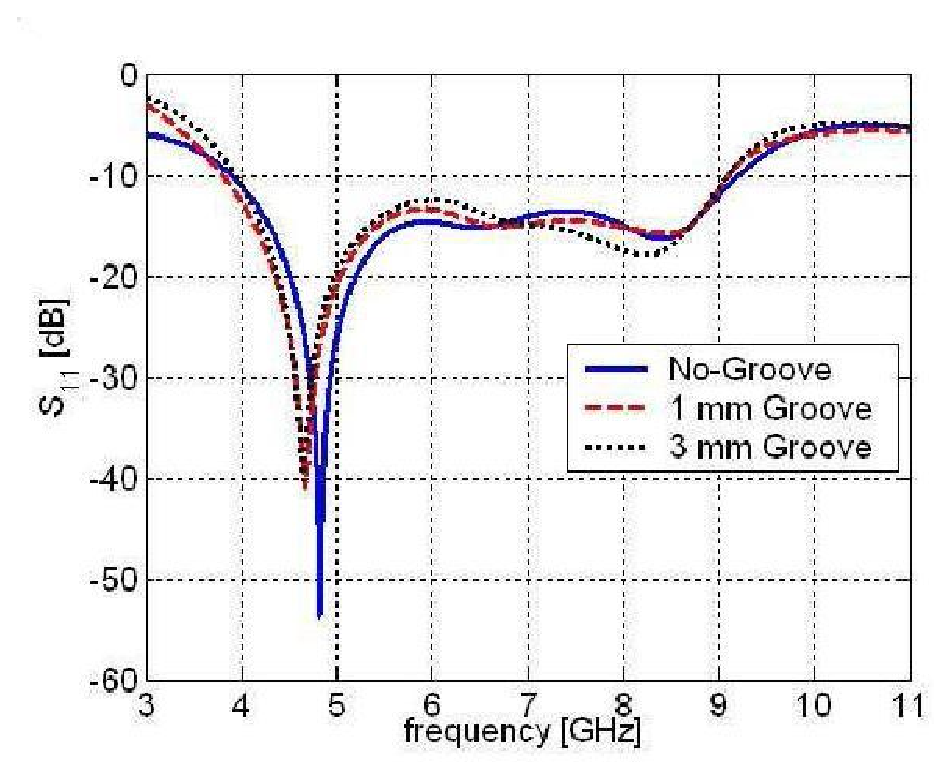
\includegraphics[width=8cm]{pict/power_reflection}
  \caption{The power reflection coefficient versus groove size. \red{Every figure caption should be fully justified and end with a period. Use 10 pt font.}}
  \label{fig:power_reflection}
  \end{center}
\end{figure}
%

Table titles should be fully justified above the table. Titles should have the following form: ``Table \#: Table title'', as shown in Table \ref{tab:greek}. Leave one blank line before and after each table or figure. Do not include a period ``.'' at the end of a table title. For a large table or a large figure, is it accepted to have them stretched to cover both columns (one column format).
%
\begin{table}
\begin{center}
\caption{First five letters of the Greek alphabet}
\begin{tabularx}{\columnwidth}{X|X|X}
%
\hline
%
{\bf Uppercase} & {\bf Lowercase} & {\bf Name}\\
%
\hline
A & $\alpha$ & ALPHA\\
\hline
B & $\beta$ & BETA\\
\hline
$\Gamma$ & $\gamma$ & GAMMA\\
\hline
$\Delta$ & $\delta$ & DELTA\\
\hline
E & $\epsilon$ & EPSILON\\
\hline
%
\end{tabularx}
\label{tab:greek}
\end{center}
\end{table}
%
\subsection{Reference formatting}
%
Please use the format of example references at the end of this document. For paper titles, only capitalize the first word, except for proper nouns and element symbols. For book titles, the first letter of each word needs to be capitalized. The first name and middle name of author(s) need to be initialized and separated by a space. \red{For all references, the publication year should always be at the end followed by a period. All text of the references should be fully justified and to the right of the reference number. Use font size 10 pt for references.} In the body of the paper, references should be cited as \cite{elsherbeni,1138693,opac-b1105789,4135853}
%
\section{COPYRIGHT AND RELEASE INFORMATION}
%
Permission is granted to quote short passages and reproduce figures and tables from ACES Journal issues provided the source is cited. Copies of ACES Journal articles may be made in accordance with usage permitted by Sections 107 or 108 of the U.S. Copyright Law. This consent does not extend to other kinds of copying, such as for general distribution, for advertising or promotional purposes, for creating new collective works, or for resale. The reproduction of multiple copies and the use of articles or extracts for commercial purposes require the consent of the author and specific permission from ACES.
%
\section{PUBLICATION CHARGES}
%
\red{All authors are allowed 6 printed pages per paper without charge. Mandatory page charges of \$50 a page apply to all pages in excess of 6 printed pages.} Printed copies of the Journal issues are available for a nominal fee by using the online request form or by submitting a request to the managing editor or ACES Secretary.
%
\section{CONCLUSION}
%
This document presents the formatting requirements for an ACES Journal paper ready for printing. The ACES Journal is abstracted in INSPEC, Engineering Index, DTIC, Science Citation Index Expanded, the Research Alert, and to Current Contents/Engineering, Computing \& Technology.
%
\section*{ACKNOWLEDGMENT}
%
In this section, acknowledge financial and sponsor support, if any. \red{Acknowledgement to your own institution is not proper and should not be included.}
%
\bibliographystyle{ACESJournal}
\bibliography{bibl/sample}
%
\begin{ACESbiography}{First Author Name}{pict/head_shot.pdf}
Provide a short biographical sketch of the first author here. \red{Do not precede the author name with a title (Dr., Prof., etc.).} Typical biographies include information such as education, job experience, and research interests or activities. The biography may also include a summary of ACES activities and positions held and similar information for other professional societies.

An author bio is generally one to three paragraphs long. \red{Total length of an author biographical sketch should be less than 300 words.} Headshot image size should be 1.2 $\times$ 1 inch.
\end{ACESbiography}
%
\begin{ACESbiography}{Second Author Name}{pict/head_shot.pdf}
Provide a short biographical sketch of the first author here. \red{Do not precede the author name with a title (Dr., Prof., etc.).} Typical biographies include information such as education, job experience, and research interests or activities. The biography may also include a summary of ACES activities and positions held and similar information for other professional societies.

An author bio is generally one to three paragraphs long. \red{Total length of an author biographical sketch should be less than 300 words.} Headshot image size should be 1.2 $\times$ 1 inch.
\end{ACESbiography}
%
%\layout
%
\end{document}
